

%%%%%%%%%%%%%%%%%%%%%%%%%%%%%%%%%%%%%%%%%%%%%%%%%%%%%%%%%%%%%%%%%%%%%%%%%%%

%%  EXTENDED LaTeX

%%%%%%%%%%%%%%%%%%%%%%%%%%%%%%%%%%%%%%%%%%%%%%%%%%%%%%%%%%%%%%%%%%%%%%%%%%%

%% Fait :

%% Révisions maketitle, sections, note \section* (absence numérotation et non
%% incrémentation)

%% notes sur abstract

%% pb césure des mots en français (marche sous linux mais donne sig-nal sous
%% Windows !.  graphicx, includegraphics, width, angle (pb comment exporter un
%% graphique excel au format jpg ou png ?  environnement figure (+ caption en
%% dessous)).

%% Pas fait divers environnements (sauf center pour includegraphics) ni tabular et
%% table.

%% Mettre sur le site du labo ce fichier PDF avec la présentation du cours.
%% L'exporter en XML ? Ajouter le plan des séances à venir ?




\section{Introduire des graphiques}
\label{graphics}

\vfill

Deux points indépendants :

\begin{itemize}
\item L'insertion d'une image dans un document \LaTeX\ 
  (cf.~\ref{includegraphics}).
\item Le positionnement d'une figure et de son titre dans le document ainsi que
  sa numérotation automatique (cf.~\ref{figure}).
\end{itemize}

\vfill



\section{Formats d'images reconnus}
\label{sec:formats-graphiques}


\vfill
\begin{itemize}
\item EPS (Embedded PostScript), PDF $\Rightarrow$ Formats vectoriels
\item PNG, JPG $\Rightarrow$ Formats bitmap
\end{itemize}


\begin{description}
\item[EPS] Nécessite de convertir le fichier \LaTeX\ en DVI puis en
  Postscript
\item[PDF, PNG, JPG] Nécessite de passer directement du fichier
  \LaTeX\ au format PDF
\end{description}

\vfill

\section{Rappel sur la création de documents PDF}

\vfill{}

\begin{description}
\item[classique] \LaTeX\ $\Rightarrow$ DVI $\Rightarrow$ PS $\Rightarrow$ PDF
%\item[dvipdfm] \LaTeX\ $\Rightarrow$ DVI $\Rightarrow$ PDF
\item[pdflatex] \LaTeX\ $\Rightarrow$ PDF
\end{description}

Nous utiliserons uniquement la dernière méthode. Elle permet d'insérer
des graphiques dans des formats assez fréquents sous Windows et Mac OS
(JPEG, PNG, mais aussi PDF).

% La méthode classique peut être intéressante pour ceux qui utilisent l'extension
% \emph{PSTricks} qui fournit des outils intéressants pour la génération de
% graphes. Elle nécessite cependant l'usage de graphiques au format Postscript
% (peu utilisés sous Windows, en tout cas peu connus des
% utilisateurs\footnote{Postscript est le format de prédilection utilisé sous
%   Unix})

\vfill{}

\section{Insérer une image}
\label{includegraphics}

\vfill

\begin{boxedminipage}{\textwidth}
  Au choix (en fonction de la méthode de création du fichier PDF et
  \emph{par conséquent} des formats de graphiques que vous utilisez :
\begin{verbatim}

\usepackage[pdftex]{graphicx} ou \usepackage[dvips]{graphicx}

puis :
\includegraphics[width=.8\textwidth, angle=90]{repertoire/nom-du-fichier}

\end{verbatim}
\end{boxedminipage}

\begin{itemize}
\item Attention au \og x \fg de \emph{graphicx}, qu'on ne retrouve pas
  par contre dans \verb1\includegraphics{}1.
\item Si on omet l'extension pour le fichier \og nom-du-fichier \fg, c'est
  \LaTeX\ qui sélectionnera l'extension en fonction de la méthode utilisée
  (pdftex, dvips) et des fichiers qu'il trouvera sur le disque.
\item \og width \fg détermine la largeur de l'image. \verb1\textwidth1
  correspond à la largeur du texte. Ceci permet d'utiliser une largeur
  relative et pas absolue. On peut aussi utiliser des largeurs
  absolues (par exemple \verb1width=8cm1).
\item \og angle \fg détermine l'angle de l'image (on peut donc l'orienter à
  volonté, par exemple dans le sens de la hauteur de la page)
\item Le plus simple est de stocker les images dans le répertoire
  courant ou des sous-répertoires du répertoire courant mais il est
  aussi possible de configurer \LaTeX\ pour qu'il aille chercher
  automatiquement certains graphiques dans un répertoire commun. Nous
  n'utiliserons pas cette fonctionnalité.
\end{itemize} 


\vfill

\section{La notion de flottant}
\label{figure}

\vfill

\begin{boxedminipage}{\textwidth}
\begin{verbatim}
\begin{figure}[tbph]
  \includegraphics[width=.8\textwidth, angle=90]{nom-du-fichier}
\caption{Titre du graphique}
\end{figure}
\end{verbatim}
\end{boxedminipage}

\begin{itemize}
\item L'environnement \emph{figure} déclare que le graphique à insérer est un
  objet flottant. C'est donc à \LaTeX\ de se charger de son positionnement sur
  la page.
  \begin{itemize}
  \item On peut indiquer à \LaTeX\ que l'on souhaite que le graphique soit
    plutôt en haut d'une page (top = t), en bas d'une page (bottom = b), qu'il
    prenne une page entière (page = p) ou qu'il soit positionné à l'endroit de
    l'appel (here = h).
  \item On peut indiquer plusieurs choix possible dans l'ordre de préférence
    mais, si l'on n'indique qu'un seul choix, \LaTeX\ ne le positionnera pas
    nécessairement tel qu'indiqué (il décide de ce qui est le mieux pour une
    apparence générale optimale en fonction des dimensions du graphique et de la
    quantité de texte sur la page, tout en essayant de prendre en compte les
    souhaits du rédacteur).
  \item Notamment : [h] seul ne force pas \LaTeX\ à positionner
    l'objet à l'endroit de l'appel. Il existe une extension
    \emph{float} qui propose une option [H] qui permet de ne pas
    réellement faire \og flotter \fg les flottants (nous ne la verrons
    pas ensemble et, dans la plupart des situations, il est
    déconseillé de l'utiliser car \LaTeX\ doit pouvoir adapter le
    positionnement à ses critères typographiques de mise en page).
  \end{itemize}
\end{itemize}

\vfill


\section{Centrer un graphique sur la page}
\label{figure}

\vfill

On inclut simplement l'instruction \verb1\includegraphics1 dans un
environnement \verb1center1.

\begin{boxedminipage}{\textwidth}
\begin{verbatim}
\begin{figure}[tbph]
  \begin{center}
    \includegraphics[width=.8\textwidth, angle=90]{nom-du-fichier}
  \end{center}
\caption{Titre du graphique}
\end{figure}
\end{verbatim}
\end{boxedminipage}

\vfill

\section{Les titres de graphiques}
\label{sec:titres-graphes}

\vfill

\begin{itemize}
\item L'instruction \verb1\caption{...}1 indique le titre du graphique. Le
  graphique sera numéroté automatiquement
\item Noter l'influence du choix de la langue sur la composition du titre.
\item Noter également que le titre d'un graphique DOIT être positionné
  en-dessous du graphique (contrairement à un tableau). Donc
  \verb1\caption{}1 doit être positionné après l'appel à
  \verb1\includegraphics{}1. \LaTeX\ ne positionne pas automatiquement
  le titre en-dessous du graphique mais il existe des extensions qui
  le font (cf.~\emph{float} et \emph{caption2}).
\end{itemize}
\vfill


\section{Un exemple de graphique flottant}


\begin{figure}[H]
  \centering
  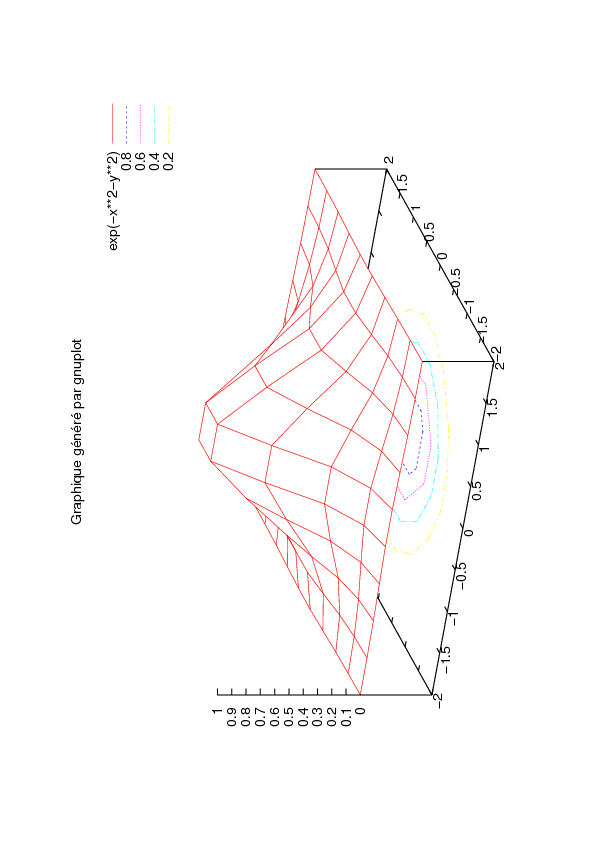
\includegraphics[width=.5\textwidth, angle=-90]{material/graphe}
  \caption{Un exemple de graphique flottant}
  \label{float}
\end{figure}


\section{Et celui d'un graphique non-flottant}

\begin{center}
  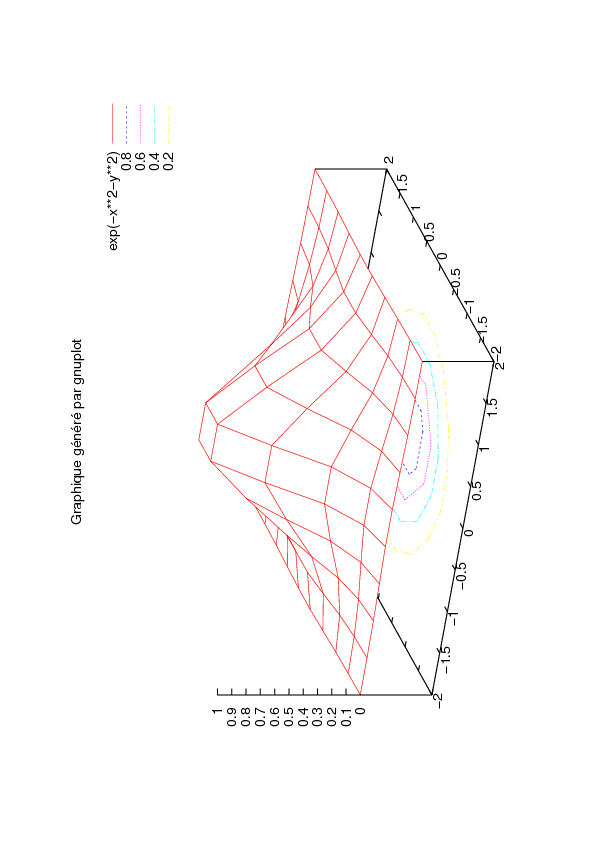
\includegraphics[width=.5\textwidth, angle=-90]{material/graphe}
  \label{nofloat}
\end{center}

Le seul moyen pour attribuer un titre à un graphique est de le faire
flotter (c'est voulu). La commande \verb1\caption1 ne peut pas être
utilisée en dehors de l'environnement \verb1figure1. Il est de toutes
façons recommandé de \emph{toujours} faire flotter les graphiques.


\section{Faire référence à un graphique}

\begin{itemize}
\item Ne fonctionne que pour les graphiques flottants (i.e. ceux à qui on
  attribue un numéro, par exemple, le graphique \ref{float}). S'ils ne flottent
  pas (par exemple le second graphique dans notre exemple), c'est le numéro de
  section (cf.  section \ref{nofloat}) qui sera utilisé par l'appel
  \verb1\ref{...}1. On peut bien sûr utiliser également le numéro de page (cf.
  page \pageref{nofloat}).
\item \verb1\label{nom}1 : attribue un label au graphique.
  \begin{itemize}
  \item En général, on fait précéder les labels des graphiques de
    \emph{\selectlanguage{english}fig:} (pour \emph{figure}, mais c'est juste
    une convention d'usage), par exemple \verb1\label{fig:data}1.
  \end{itemize}
\item \verb1\ref{nom}1 : effectue un renvoi vers le numéro du graphique qui
  correspond au repère \emph{nom}.
\item Pour les graphiques flottants (Attention, s'ils ne flottent pas,
  ils ne disposent pas d'un numéro ; on peut cepedendant renvoyer à la
  page sur laquelle ils apparaissent), il convient de situer l'appel
  \verb1\label{nom}1 à l'intérieur de l'environnement \emph{figure},
  juste après la commande \verb1\caption{}1.

  \begin{exemple}[H]
    \caption{Référence à un graphique}
    \label{ex:reftab}
\begin{verbatim}
\begin{figure}
  \includegraphics[width=.5\textwidth, angle=-90]{fichier}
  \caption{Titre attribué au graphique.}
  \label{fig:data}.
\end{figure}
\end{verbatim}
  \end{exemple}
  
\item \verb1\pageref{nom}1 : effectue un renvoi vers le numéro de la page qui
  correspond au repère \emph{nom}. Pour le reste, il fonctionne exactement de la
  même manière que \verb1\ref1.
\end{itemize}


Par exemple, le renvoi à ce graphique se traduirait par :

\begin{exemple}[H]
  \caption{Référence à un graphique}
  \label{ex:reftab}
\begin{verbatim}
On voit dans la Figure~/ref{fig:data}, p.\pageref{fig:data}...
\end{verbatim}
\end{exemple}


Notez l'usage du caractère \og \verb1~1 \fg (tilde) qui permet
d'insérer un espace insécable (pour obtenir ce caractère, on utilise
AltGr+2 sur un PC et Command+SHIFT+N sur un Mac).
